\subsection{filter\_\-t Struct Reference}
\label{structfilter__t}\index{filter\_\-t@{filter\_\-t}}
{\tt \#include $<$bpm\_\-dsp.h$>$}

Collaboration diagram for filter\_\-t:\nopagebreak
\begin{figure}[H]
\begin{center}
\leavevmode
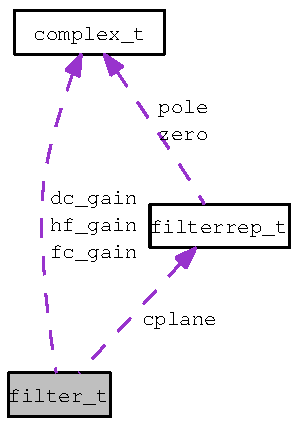
\includegraphics[width=89pt]{structfilter__t__coll__graph}
\end{center}
\end{figure}


\subsubsection{Detailed Description}
The filter structure. 

Definition at line 437 of file bpm\_\-dsp.h.\subsubsection*{Data Fields}
\begin{CompactItemize}
\item 
char {\bf name} [80]
\item 
unsigned int {\bf options}
\item 
int {\bf order}
\item 
double {\bf fs}
\item 
double {\bf f1}
\item 
double {\bf f2}
\item 
double {\bf alpha1}
\item 
double {\bf alpha2}
\item 
double {\bf w\_\-alpha1}
\item 
double {\bf w\_\-alpha2}
\item 
double {\bf cheb\_\-ripple}
\item 
double {\bf Q}
\item 
double {\bf gauss\_\-cutoff}
\item 
{\bf complex\_\-t} {\bf dc\_\-gain}
\item 
{\bf complex\_\-t} {\bf fc\_\-gain}
\item 
{\bf complex\_\-t} {\bf hf\_\-gain}
\item 
double {\bf gain}
\item 
{\bf filterrep\_\-t} $\ast$ {\bf cplane}
\item 
int {\bf nxc}
\item 
double {\bf xc} [MAXPZ+1]
\item 
int {\bf nxc\_\-ac}
\item 
double {\bf xc\_\-ac} [MAXPZ+1]
\item 
int {\bf nyc}
\item 
double {\bf yc} [MAXPZ+1]
\item 
int {\bf nyc\_\-ac}
\item 
double {\bf yc\_\-ac} [MAXPZ+1]
\item 
double {\bf xv} [MAXPZ+1]
\item 
double {\bf xv\_\-ac} [MAXPZ+1]
\item 
double {\bf yv} [MAXPZ+1]
\item 
double {\bf yv\_\-ac} [MAXPZ+1]
\item 
int {\bf ns}
\item 
double $\ast$ {\bf wfbuffer}
\end{CompactItemize}


\subsubsection{Field Documentation}
\index{filter\_\-t@{filter\_\-t}!name@{name}}
\index{name@{name}!filter_t@{filter\_\-t}}
\paragraph[name]{\setlength{\rightskip}{0pt plus 5cm}char {\bf filter\_\-t::name}[80]}\hfill\label{structfilter__t_420d5f6fd6f7b83fb674fe5a81c18425}


The filter's name 

Definition at line 438 of file bpm\_\-dsp.h.

Referenced by create\_\-filter(), and print\_\-filter().\index{filter\_\-t@{filter\_\-t}!options@{options}}
\index{options@{options}!filter_t@{filter\_\-t}}
\paragraph[options]{\setlength{\rightskip}{0pt plus 5cm}unsigned int {\bf filter\_\-t::options}}\hfill\label{structfilter__t_f1f1d9266ba72eda6685c631f4dde41f}


type and option bits for filter 

Definition at line 440 of file bpm\_\-dsp.h.

Referenced by apply\_\-filter(), calculate\_\-filter\_\-coefficients(), create\_\-filter(), create\_\-resonator\_\-representation(), create\_\-splane\_\-representation(), gaussian\_\-filter\_\-coeffs(), normalise\_\-filter(), print\_\-filter(), and zplane\_\-transform().\index{filter\_\-t@{filter\_\-t}!order@{order}}
\index{order@{order}!filter_t@{filter\_\-t}}
\paragraph[order]{\setlength{\rightskip}{0pt plus 5cm}int {\bf filter\_\-t::order}}\hfill\label{structfilter__t_300a7f45bc8727f2c77cf1d9845deb96}


filter order 

Definition at line 441 of file bpm\_\-dsp.h.

Referenced by create\_\-filter(), and create\_\-splane\_\-representation().\index{filter\_\-t@{filter\_\-t}!fs@{fs}}
\index{fs@{fs}!filter_t@{filter\_\-t}}
\paragraph[fs]{\setlength{\rightskip}{0pt plus 5cm}double {\bf filter\_\-t::fs}}\hfill\label{structfilter__t_fcb71153474c026e4af9eb79e134272c}


sampling frequency 

Definition at line 443 of file bpm\_\-dsp.h.

Referenced by create\_\-filter(), and gaussian\_\-filter\_\-coeffs().\index{filter\_\-t@{filter\_\-t}!f1@{f1}}
\index{f1@{f1}!filter_t@{filter\_\-t}}
\paragraph[f1]{\setlength{\rightskip}{0pt plus 5cm}double {\bf filter\_\-t::f1}}\hfill\label{structfilter__t_ee11cdb8bd177a80af5a8145ef2994a7}


first frequency ( left edge for bandpass/stop ) 

Definition at line 444 of file bpm\_\-dsp.h.

Referenced by create\_\-filter(), and gaussian\_\-filter\_\-coeffs().\index{filter\_\-t@{filter\_\-t}!f2@{f2}}
\index{f2@{f2}!filter_t@{filter\_\-t}}
\paragraph[f2]{\setlength{\rightskip}{0pt plus 5cm}double {\bf filter\_\-t::f2}}\hfill\label{structfilter__t_f20ed86d13f7d772b34d24fdad574d98}


right edge for bandpass/stop ( undef for low/highpass ) 

Definition at line 445 of file bpm\_\-dsp.h.

Referenced by create\_\-filter().\index{filter\_\-t@{filter\_\-t}!alpha1@{alpha1}}
\index{alpha1@{alpha1}!filter_t@{filter\_\-t}}
\paragraph[alpha1]{\setlength{\rightskip}{0pt plus 5cm}double {\bf filter\_\-t::alpha1}}\hfill\label{structfilter__t_cc6b5340d5c29772295c9e9a77996875}


rescaled f1 

Definition at line 447 of file bpm\_\-dsp.h.

Referenced by calculate\_\-filter\_\-coefficients(), create\_\-filter(), and create\_\-resonator\_\-representation().\index{filter\_\-t@{filter\_\-t}!alpha2@{alpha2}}
\index{alpha2@{alpha2}!filter_t@{filter\_\-t}}
\paragraph[alpha2]{\setlength{\rightskip}{0pt plus 5cm}double {\bf filter\_\-t::alpha2}}\hfill\label{structfilter__t_8124f521ac4d25e9afbca612f8afa202}


rescaled f2 

Definition at line 448 of file bpm\_\-dsp.h.

Referenced by calculate\_\-filter\_\-coefficients(), and create\_\-filter().\index{filter\_\-t@{filter\_\-t}!w\_\-alpha1@{w\_\-alpha1}}
\index{w\_\-alpha1@{w\_\-alpha1}!filter_t@{filter\_\-t}}
\paragraph[w\_\-alpha1]{\setlength{\rightskip}{0pt plus 5cm}double {\bf filter\_\-t::w\_\-alpha1}}\hfill\label{structfilter__t_dc08473e572d2bb1b6442d7ccda22d7a}


warped alpha1 

Definition at line 450 of file bpm\_\-dsp.h.

Referenced by create\_\-filter(), and normalise\_\-filter().\index{filter\_\-t@{filter\_\-t}!w\_\-alpha2@{w\_\-alpha2}}
\index{w\_\-alpha2@{w\_\-alpha2}!filter_t@{filter\_\-t}}
\paragraph[w\_\-alpha2]{\setlength{\rightskip}{0pt plus 5cm}double {\bf filter\_\-t::w\_\-alpha2}}\hfill\label{structfilter__t_b1712c2f6e445670dd8e4063f2e281ad}


warped alpha2 

Definition at line 451 of file bpm\_\-dsp.h.

Referenced by create\_\-filter(), and normalise\_\-filter().\index{filter\_\-t@{filter\_\-t}!cheb\_\-ripple@{cheb\_\-ripple}}
\index{cheb\_\-ripple@{cheb\_\-ripple}!filter_t@{filter\_\-t}}
\paragraph[cheb\_\-ripple]{\setlength{\rightskip}{0pt plus 5cm}double {\bf filter\_\-t::cheb\_\-ripple}}\hfill\label{structfilter__t_674643ee7b183192df19cd3cd7e38a3d}


ripple for chebyshev filters 

Definition at line 453 of file bpm\_\-dsp.h.

Referenced by create\_\-filter(), and create\_\-splane\_\-representation().\index{filter\_\-t@{filter\_\-t}!Q@{Q}}
\index{Q@{Q}!filter_t@{filter\_\-t}}
\paragraph[Q]{\setlength{\rightskip}{0pt plus 5cm}double {\bf filter\_\-t::Q}}\hfill\label{structfilter__t_1a2c1f97d417a58cb58346906afc8205}


Q factor for resonators 

Definition at line 454 of file bpm\_\-dsp.h.

Referenced by create\_\-filter(), and create\_\-resonator\_\-representation().\index{filter\_\-t@{filter\_\-t}!gauss\_\-cutoff@{gauss\_\-cutoff}}
\index{gauss\_\-cutoff@{gauss\_\-cutoff}!filter_t@{filter\_\-t}}
\paragraph[gauss\_\-cutoff]{\setlength{\rightskip}{0pt plus 5cm}double {\bf filter\_\-t::gauss\_\-cutoff}}\hfill\label{structfilter__t_bb943262c0d73b7dc911fc5ec4f155a6}


gaussian filter cutoff parameter 

Definition at line 455 of file bpm\_\-dsp.h.

Referenced by create\_\-filter(), and gaussian\_\-filter\_\-coeffs().\index{filter\_\-t@{filter\_\-t}!dc\_\-gain@{dc\_\-gain}}
\index{dc\_\-gain@{dc\_\-gain}!filter_t@{filter\_\-t}}
\paragraph[dc\_\-gain]{\setlength{\rightskip}{0pt plus 5cm}{\bf complex\_\-t} {\bf filter\_\-t::dc\_\-gain}}\hfill\label{structfilter__t_1fb8ef235aebd042e645d032a45e71df}


Complex DC gain of the filter 

Definition at line 457 of file bpm\_\-dsp.h.

Referenced by calculate\_\-filter\_\-coefficients(), and print\_\-filter().\index{filter\_\-t@{filter\_\-t}!fc\_\-gain@{fc\_\-gain}}
\index{fc\_\-gain@{fc\_\-gain}!filter_t@{filter\_\-t}}
\paragraph[fc\_\-gain]{\setlength{\rightskip}{0pt plus 5cm}{\bf complex\_\-t} {\bf filter\_\-t::fc\_\-gain}}\hfill\label{structfilter__t_be3e7477ffd82a35ab7c0e7dcdc4a314}


Complex Center frequency gain of filter 

Definition at line 458 of file bpm\_\-dsp.h.

Referenced by calculate\_\-filter\_\-coefficients(), and print\_\-filter().\index{filter\_\-t@{filter\_\-t}!hf\_\-gain@{hf\_\-gain}}
\index{hf\_\-gain@{hf\_\-gain}!filter_t@{filter\_\-t}}
\paragraph[hf\_\-gain]{\setlength{\rightskip}{0pt plus 5cm}{\bf complex\_\-t} {\bf filter\_\-t::hf\_\-gain}}\hfill\label{structfilter__t_a383fcf8e8345bd268d40a374276bb0f}


Complex High frequency (fNy) gain of filter 

Definition at line 459 of file bpm\_\-dsp.h.

Referenced by calculate\_\-filter\_\-coefficients(), and print\_\-filter().\index{filter\_\-t@{filter\_\-t}!gain@{gain}}
\index{gain@{gain}!filter_t@{filter\_\-t}}
\paragraph[gain]{\setlength{\rightskip}{0pt plus 5cm}double {\bf filter\_\-t::gain}}\hfill\label{structfilter__t_9f8ff8688cc79f123f63209d62073677}


Actual Filter gain 

Definition at line 460 of file bpm\_\-dsp.h.

Referenced by apply\_\-filter(), calculate\_\-filter\_\-coefficients(), gaussian\_\-filter\_\-coeffs(), and print\_\-filter().\index{filter\_\-t@{filter\_\-t}!cplane@{cplane}}
\index{cplane@{cplane}!filter_t@{filter\_\-t}}
\paragraph[cplane]{\setlength{\rightskip}{0pt plus 5cm}{\bf filterrep\_\-t}$\ast$ {\bf filter\_\-t::cplane}}\hfill\label{structfilter__t_d60ad283b3847bcf61069cb0aecb3a84}


pointer to complex filter representation, poles and zeros 

Definition at line 462 of file bpm\_\-dsp.h.

Referenced by calculate\_\-filter\_\-coefficients(), create\_\-filter(), delete\_\-filter(), and print\_\-filter().\index{filter\_\-t@{filter\_\-t}!nxc@{nxc}}
\index{nxc@{nxc}!filter_t@{filter\_\-t}}
\paragraph[nxc]{\setlength{\rightskip}{0pt plus 5cm}int {\bf filter\_\-t::nxc}}\hfill\label{structfilter__t_0a4cebb1e641ab50077f260ad11c7788}


number of x coefficients 

Definition at line 464 of file bpm\_\-dsp.h.

Referenced by apply\_\-filter(), calculate\_\-filter\_\-coefficients(), gaussian\_\-filter\_\-coeffs(), and print\_\-filter().\index{filter\_\-t@{filter\_\-t}!xc@{xc}}
\index{xc@{xc}!filter_t@{filter\_\-t}}
\paragraph[xc]{\setlength{\rightskip}{0pt plus 5cm}double {\bf filter\_\-t::xc}[MAXPZ+1]}\hfill\label{structfilter__t_22b9df0209c051f2ddc148486e7d6f8a}


pointer to array of x coefficients 

Definition at line 465 of file bpm\_\-dsp.h.

Referenced by apply\_\-filter(), calculate\_\-filter\_\-coefficients(), gaussian\_\-filter\_\-coeffs(), and print\_\-filter().\index{filter\_\-t@{filter\_\-t}!nxc\_\-ac@{nxc\_\-ac}}
\index{nxc\_\-ac@{nxc\_\-ac}!filter_t@{filter\_\-t}}
\paragraph[nxc\_\-ac]{\setlength{\rightskip}{0pt plus 5cm}int {\bf filter\_\-t::nxc\_\-ac}}\hfill\label{structfilter__t_92369adf50700705324f0ead36ec800c}


number of anti-causal x coefficients 

Definition at line 467 of file bpm\_\-dsp.h.

Referenced by apply\_\-filter(), gaussian\_\-filter\_\-coeffs(), and print\_\-filter().\index{filter\_\-t@{filter\_\-t}!xc\_\-ac@{xc\_\-ac}}
\index{xc\_\-ac@{xc\_\-ac}!filter_t@{filter\_\-t}}
\paragraph[xc\_\-ac]{\setlength{\rightskip}{0pt plus 5cm}double {\bf filter\_\-t::xc\_\-ac}[MAXPZ+1]}\hfill\label{structfilter__t_7918586bf5ed32660dabe328a1f2589f}


pointer to array of anti-causal x coefficients 

Definition at line 468 of file bpm\_\-dsp.h.

Referenced by apply\_\-filter(), gaussian\_\-filter\_\-coeffs(), and print\_\-filter().\index{filter\_\-t@{filter\_\-t}!nyc@{nyc}}
\index{nyc@{nyc}!filter_t@{filter\_\-t}}
\paragraph[nyc]{\setlength{\rightskip}{0pt plus 5cm}int {\bf filter\_\-t::nyc}}\hfill\label{structfilter__t_b67b5502d78fb69739317f7330d9bf19}


number of y coefficients (for IIR filters) 

Definition at line 470 of file bpm\_\-dsp.h.

Referenced by apply\_\-filter(), calculate\_\-filter\_\-coefficients(), and print\_\-filter().\index{filter\_\-t@{filter\_\-t}!yc@{yc}}
\index{yc@{yc}!filter_t@{filter\_\-t}}
\paragraph[yc]{\setlength{\rightskip}{0pt plus 5cm}double {\bf filter\_\-t::yc}[MAXPZ+1]}\hfill\label{structfilter__t_f90b9fd76e7e0bf377a17ea23ca589f0}


pointer to array of y coefficients 

Definition at line 471 of file bpm\_\-dsp.h.

Referenced by apply\_\-filter(), calculate\_\-filter\_\-coefficients(), create\_\-filter(), and print\_\-filter().\index{filter\_\-t@{filter\_\-t}!nyc\_\-ac@{nyc\_\-ac}}
\index{nyc\_\-ac@{nyc\_\-ac}!filter_t@{filter\_\-t}}
\paragraph[nyc\_\-ac]{\setlength{\rightskip}{0pt plus 5cm}int {\bf filter\_\-t::nyc\_\-ac}}\hfill\label{structfilter__t_0efd9c9142e1de7ed343838b73c6bbca}


number of anti-causal y coefficients (for IIR filters) 

Definition at line 473 of file bpm\_\-dsp.h.\index{filter\_\-t@{filter\_\-t}!yc\_\-ac@{yc\_\-ac}}
\index{yc\_\-ac@{yc\_\-ac}!filter_t@{filter\_\-t}}
\paragraph[yc\_\-ac]{\setlength{\rightskip}{0pt plus 5cm}double {\bf filter\_\-t::yc\_\-ac}[MAXPZ+1]}\hfill\label{structfilter__t_a51fea51992b0ad09ad85a504ce2223e}


pointer to array of anti-causal y coefficients 

Definition at line 474 of file bpm\_\-dsp.h.\index{filter\_\-t@{filter\_\-t}!xv@{xv}}
\index{xv@{xv}!filter_t@{filter\_\-t}}
\paragraph[xv]{\setlength{\rightskip}{0pt plus 5cm}double {\bf filter\_\-t::xv}[MAXPZ+1]}\hfill\label{structfilter__t_26b1836d03ff46c9d76a9129ae225820}


filter x buffer, used in apply\_\-filter 

Definition at line 476 of file bpm\_\-dsp.h.

Referenced by apply\_\-filter().\index{filter\_\-t@{filter\_\-t}!xv\_\-ac@{xv\_\-ac}}
\index{xv\_\-ac@{xv\_\-ac}!filter_t@{filter\_\-t}}
\paragraph[xv\_\-ac]{\setlength{\rightskip}{0pt plus 5cm}double {\bf filter\_\-t::xv\_\-ac}[MAXPZ+1]}\hfill\label{structfilter__t_48fa496d9b7b4c496ae3209a4d8004d6}


filter x buffer, used in apply\_\-filter 

Definition at line 477 of file bpm\_\-dsp.h.

Referenced by apply\_\-filter().\index{filter\_\-t@{filter\_\-t}!yv@{yv}}
\index{yv@{yv}!filter_t@{filter\_\-t}}
\paragraph[yv]{\setlength{\rightskip}{0pt plus 5cm}double {\bf filter\_\-t::yv}[MAXPZ+1]}\hfill\label{structfilter__t_7c459fa3bbf050e6a2521cd5f7542f5d}


filter y buffer, used in apply\_\-filter 

Definition at line 479 of file bpm\_\-dsp.h.

Referenced by apply\_\-filter().\index{filter\_\-t@{filter\_\-t}!yv\_\-ac@{yv\_\-ac}}
\index{yv\_\-ac@{yv\_\-ac}!filter_t@{filter\_\-t}}
\paragraph[yv\_\-ac]{\setlength{\rightskip}{0pt plus 5cm}double {\bf filter\_\-t::yv\_\-ac}[MAXPZ+1]}\hfill\label{structfilter__t_71a724a67ac888e6aaebc3962d82b3aa}


filter y buffer, used in apply\_\-filter 

Definition at line 480 of file bpm\_\-dsp.h.

Referenced by apply\_\-filter().\index{filter\_\-t@{filter\_\-t}!ns@{ns}}
\index{ns@{ns}!filter_t@{filter\_\-t}}
\paragraph[ns]{\setlength{\rightskip}{0pt plus 5cm}int {\bf filter\_\-t::ns}}\hfill\label{structfilter__t_f90dc219ac95f6b1723622a4b7946b93}


number of samples of waveforms to be filtered 

Definition at line 482 of file bpm\_\-dsp.h.

Referenced by apply\_\-filter(), create\_\-filter(), filter\_\-impulse\_\-response(), filter\_\-step\_\-response(), and gaussian\_\-filter\_\-coeffs().\index{filter\_\-t@{filter\_\-t}!wfbuffer@{wfbuffer}}
\index{wfbuffer@{wfbuffer}!filter_t@{filter\_\-t}}
\paragraph[wfbuffer]{\setlength{\rightskip}{0pt plus 5cm}double$\ast$ {\bf filter\_\-t::wfbuffer}}\hfill\label{structfilter__t_d5ac1b6a82e84bbcda0b70c56a1011a6}


waveform buffer for filter computations, allocated once ! 

Definition at line 483 of file bpm\_\-dsp.h.

Referenced by apply\_\-filter(), create\_\-filter(), and delete\_\-filter().

The documentation for this struct was generated from the following file:\begin{CompactItemize}
\item 
bpmdsp/{\bf bpm\_\-dsp.h}\end{CompactItemize}
